\documentclass[10pt,a4paper,twoside,openright,titlepage,twocolumn]{article}
\usepackage[utf8]{inputenc}
\usepackage[T1]{fontenc}
\usepackage[ngerman]{babel,varioref}
\usepackage[left=0.7cm,right=0.7cm,top=0.7cm,bottom=0.7cm,includeheadfoot]{geometry}

\usepackage{amsmath}
\usepackage{amssymb}
\usepackage{graphicx}
\usepackage{xcolor}
\usepackage{wrapfig}
\usepackage{siunitx}
\usepackage{titlesec}
\usepackage{titlepic}
\usepackage{listings}
\usepackage[export]{adjustbox}


\graphicspath{ {./Images/} }


\definecolor{formulablue}{RGB}{219,219,255}
\newcommand{\formula}[1]{\colorbox{formulablue}{#1}}

\newcommand{\unitText}[3]{\noindent\textit{#1} : #2 [#3]}

\definecolor{refrot}{RGB}{183,28,42}
\newcommand{\refskript}[1]{\textcolor{refrot}{Skript S.#1}}



\titlespacing*{\section}{0pt}{12pt}{0pt}
\titlespacing*{\subsection}{0pt}{0pt}{0pt}
\titlespacing*{\subsubsection}{0pt}{0pt}{0pt}


\title{\vspace{50mm}EmbSys2 \\ [1ex] \large Formelsammlung}
\author{Sebastian Humbel}
\titlepic{\vspace{50mm}
\includegraphics[width=0.25\textwidth]{Elvis}}


% Code format
% Define the Gruvbox light colors
\definecolor{gruvbox_bg}{HTML}{fbf1c7}
\definecolor{gruvbox_fg}{HTML}{3c3836}
\definecolor{gruvbox_yellow}{HTML}{d79921}
\definecolor{gruvbox_red}{HTML}{cc241d}
\definecolor{gruvbox_green}{HTML}{98971a}
\definecolor{gruvbox_blue}{HTML}{458588}
\definecolor{gruvbox_purple}{HTML}{b16286}
\definecolor{gruvbox_aqua}{HTML}{689d6a}
\definecolor{gruvbox_orange}{HTML}{d65d0e}


\lstdefinestyle{cppstyle}{
	language=C++,
	basicstyle=\ttfamily\footnotesize,
	numbers=left,
	numberstyle=\tiny,
	numbersep=5pt,
	tabsize=4,
	showspaces=false,
	showstringspaces=false,
	frame=single,
	rulecolor=\color{gruvbox_fg},
	backgroundcolor=\color{white},
	keywordstyle=\color{gruvbox_orange},
	commentstyle=\color{gruvbox_aqua},
	stringstyle=\color{gruvbox_green},
	identifierstyle=\color{gruvbox_fg},
	emphstyle=\color{gruvbox_red},
	emph={int, double, string, cout, TimerHandle_t, BaseType_t, timerPWMPeripheral_t, SemaphoreHandle_t, TaskHandle_t, QueueHandle_t},
	xleftmargin=5mm,
	xrightmargin=\parindent
}



\begin{document}
	
	\maketitle
	\setlength\parindent{0pt}

	\section{Einleitung}

Echtzeitsysteme müssen innerhalb genauer Zeitvorgaben auf Ereignisse in der Umgebung reagieren.
Sie sind; reaktiv, effizient, verläslich, betriebssicher, spezifisch und real-time.

\subsection{Rechenleistung}

\formula{$\mathit{Time} = \dfrac{\mathit{Seconds}}{\mathit{Program}} = \dfrac{\mathit{Instructions}}{\mathit{Program}} \cdot \dfrac{\mathit{Clock cycles}}{Instruction} \cdot \dfrac{\mathit{Seconds}}{\mathit{Clock cycle}}$}

\subsection{Sense-Think-Act Paradigma}

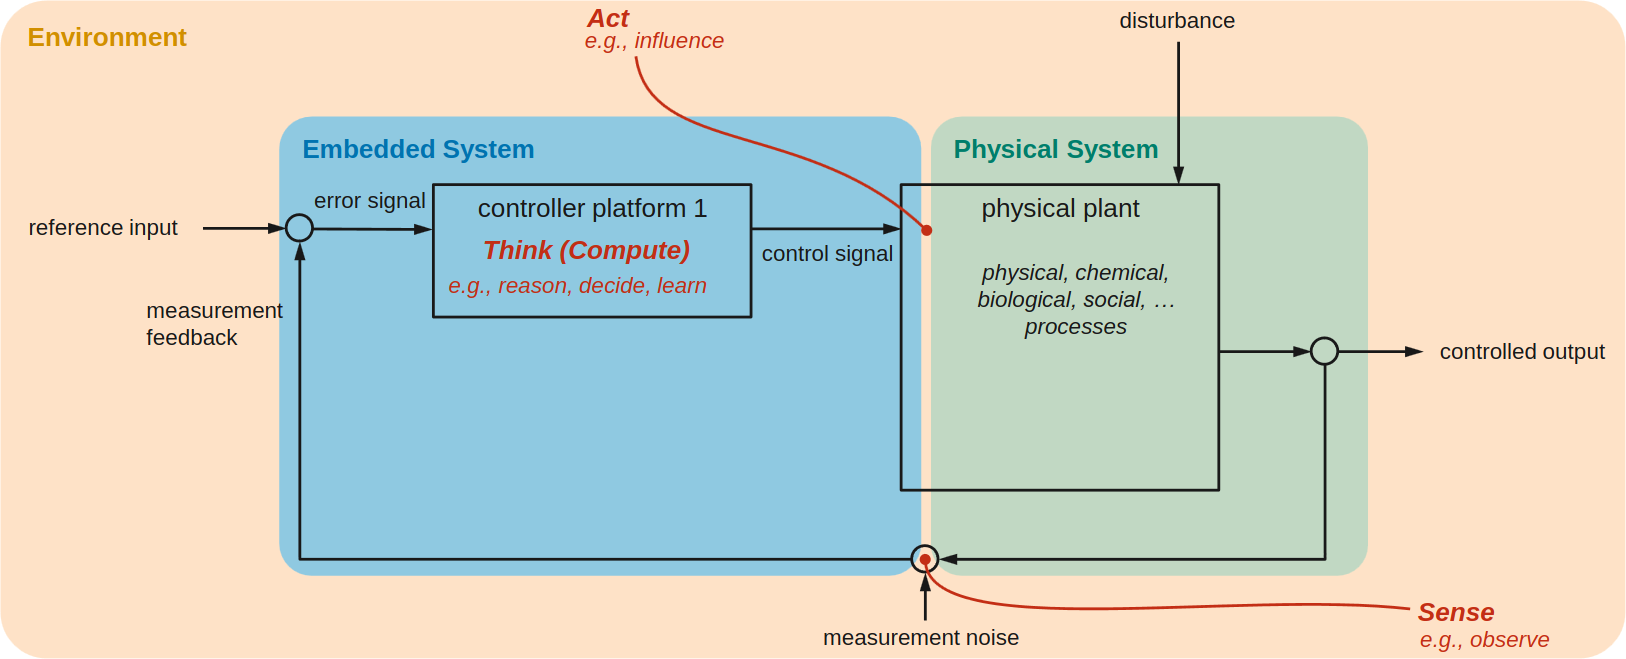
\includegraphics[width=\linewidth]{"Images/SenseThinkAct.png"}

Bei einem CPC (Cyber Physical System):

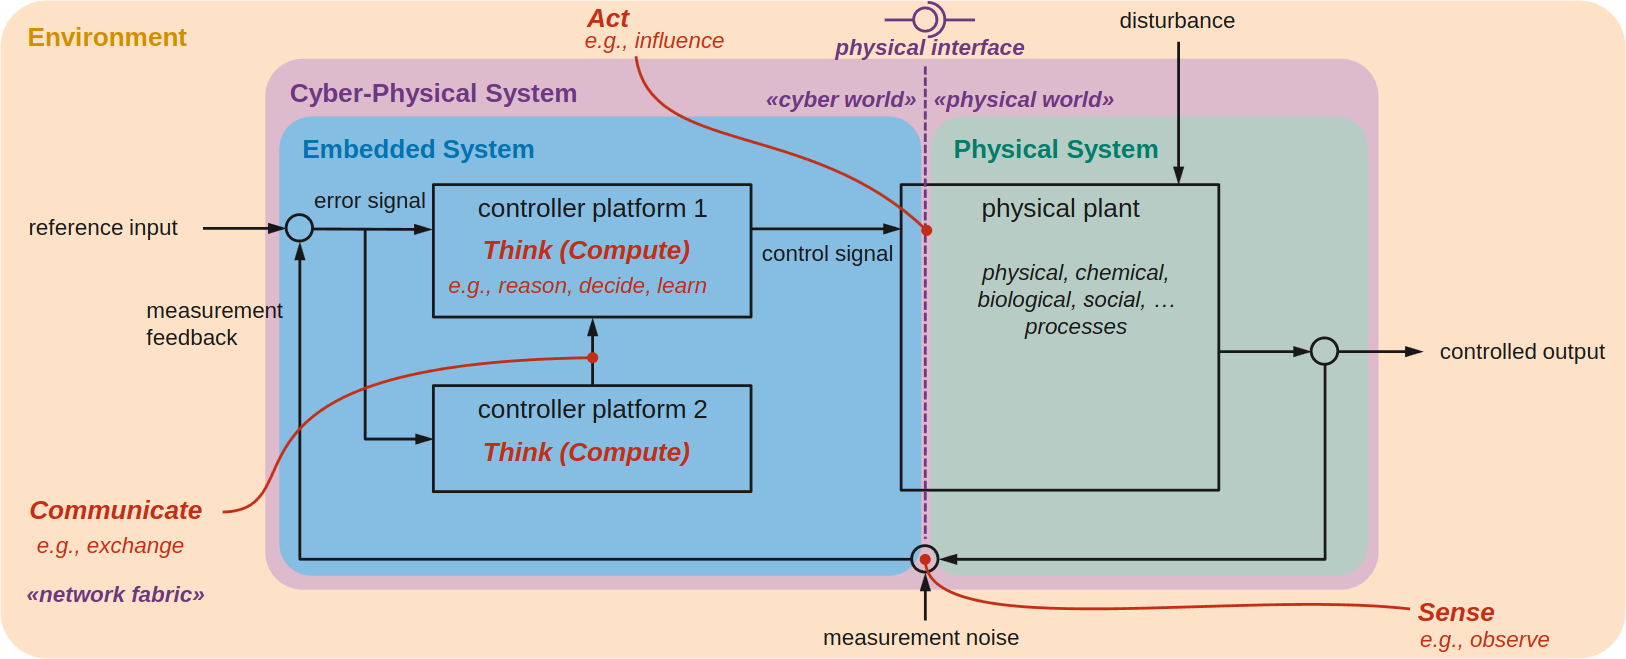
\includegraphics[width=\linewidth]{"Images/SenseThinkActCommunicate.png"}

\subsection{Schichtmodell}

\begin{center}
	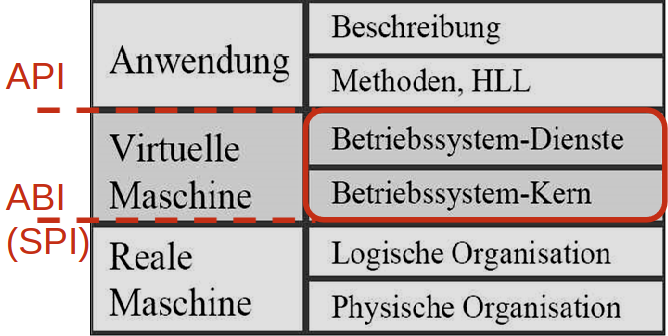
\includegraphics[width=.6\linewidth]{"Images/Schichtmodell.png"}
\end{center}

Das Betriebssystem im Schichtenmodell des Computersystems bietet der Anwendung API-Schnittstellen zur darunterliegenden realen Maschine und macht die Anwendung damit weitgehend unabhängig von der realen Maschine (CPU, Hardware, Peripherien,...).

\subsection{Entwicklungsprozess}

Unterschiedliche Möglichkeiten wie V-Modell und DevOps Lyfecycle (Loop).

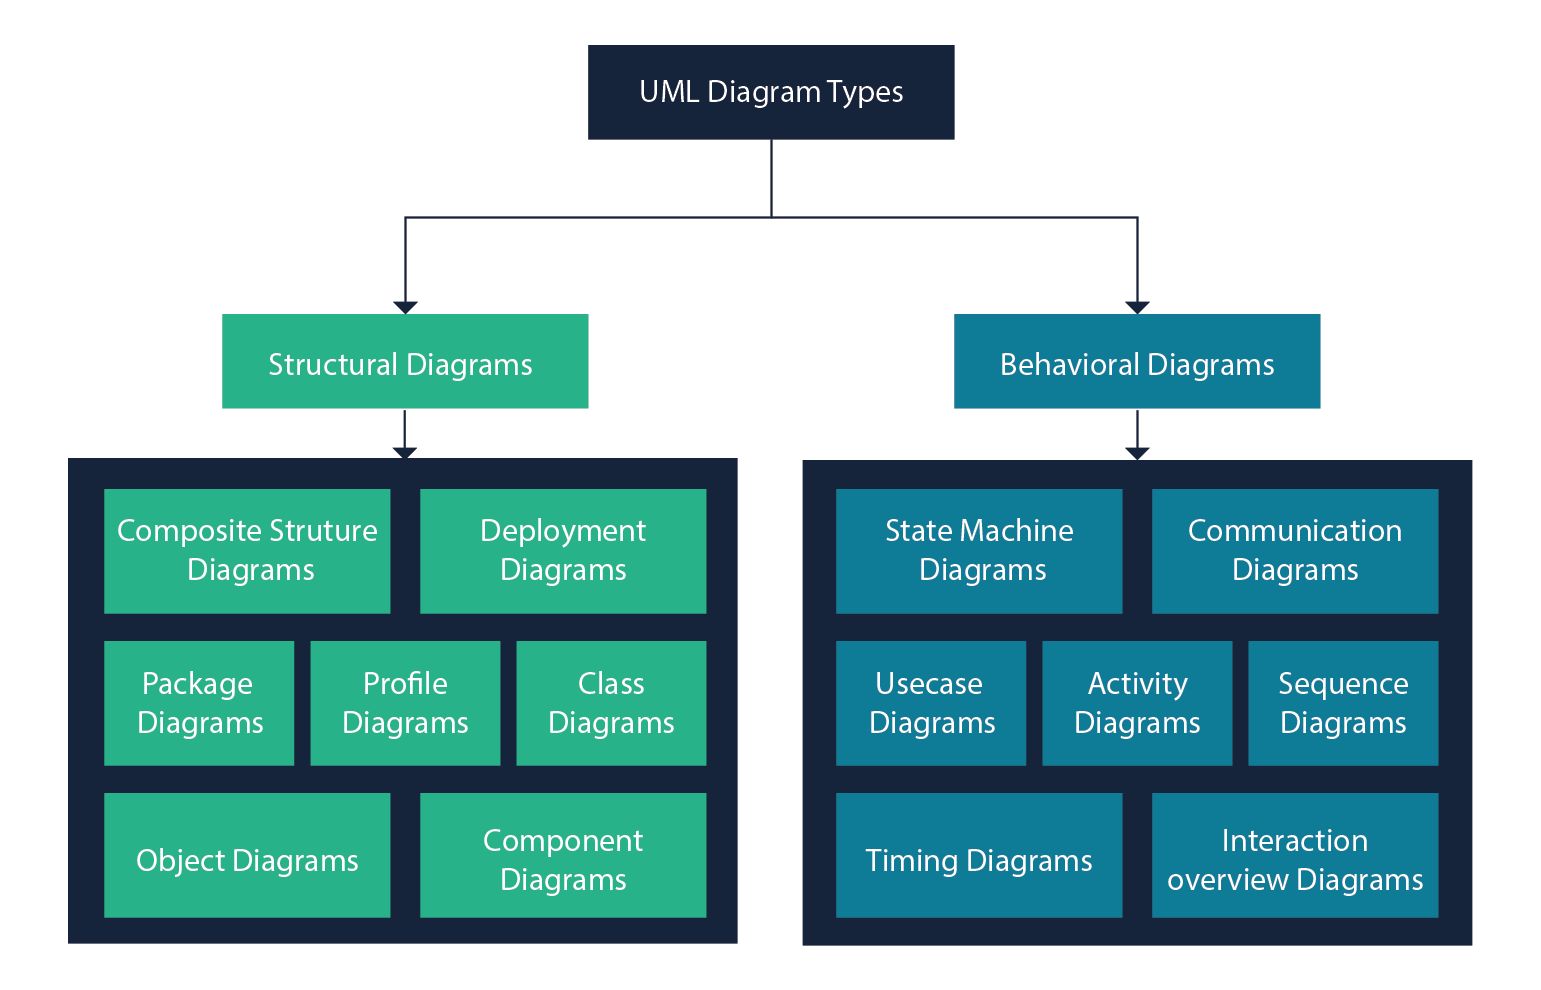
\includegraphics[width=\linewidth]{"Images/UML-Diagram-types-1.png"}

\subsection{Mikrocontroller-Organisation}

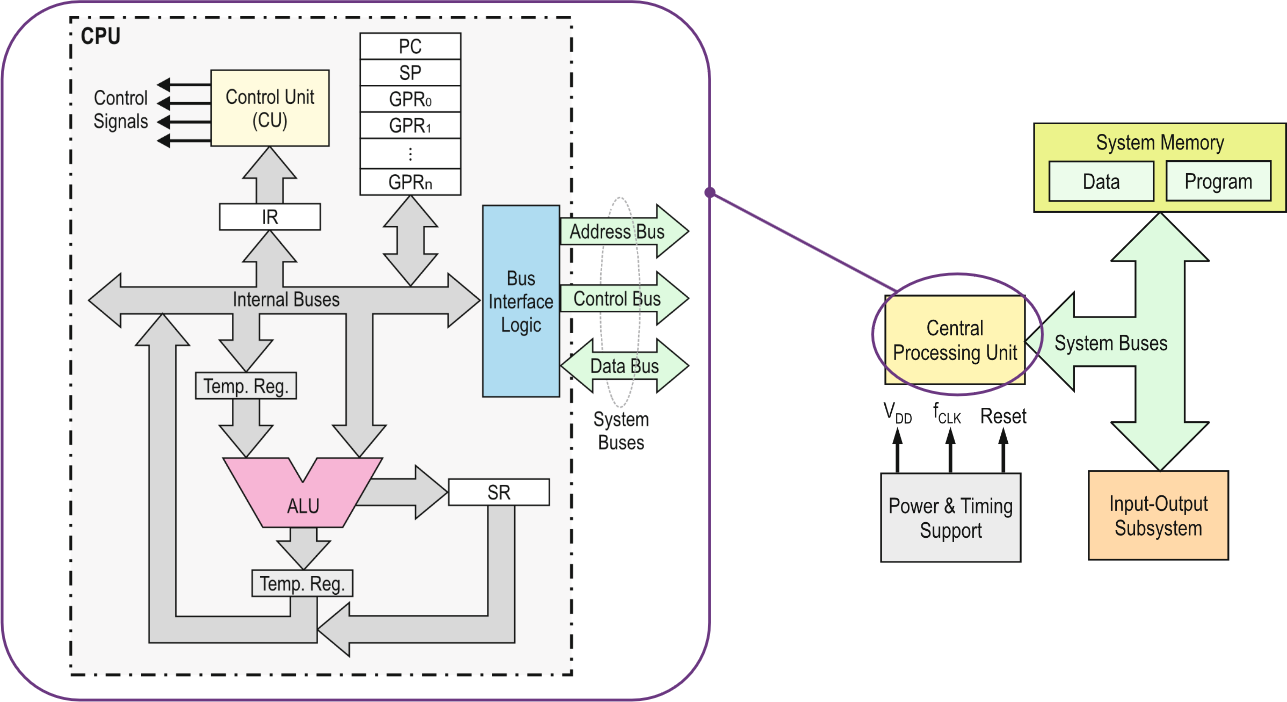
\includegraphics[width=\linewidth]{"Images/MikrocontrollerOrganisation.png"}

\subsubsection{System Komponenten}

\begin{itemize}
	\itemsep-.5em 
	\item \textit{NVIC}: Nested Vectored Interrupt Controller, provides configurable interrupt handling abilities to the processor.
	\item \textit{SYSTICK}: System timer, 24-bit down-counter, automatic reload.
	\item \textit{MPU}: Memory Protection Unit, Zugriffsregeln für Privileged Access und User Program Access, wirft Exceptions.
	\item \textit{FPU}: Floating Point Unit, erweiterter Befehlssatz auf DSP.
\end{itemize}

	\section{Betriebssysteme}

	\section{Interprozesskommunikation}

\subsection{Semaphore}

Semaphor ist ein Signalisierungsmechanismus (signaling mechanism), bestehend aus einer P-Operation (proberen, prüfen, reservieren) und V-Opration (verhogen, erhöhen, freigeben).

Binäre Semaphore:

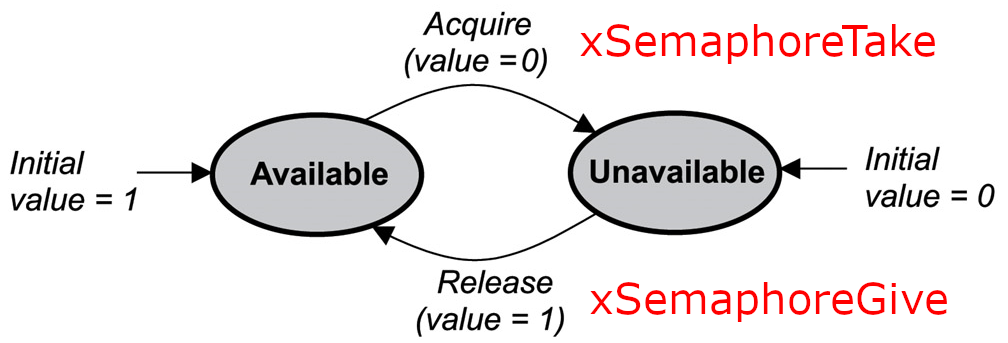
\includegraphics[width=.9\linewidth]{Binary_Semaphore.png}

Counting Semaphore:

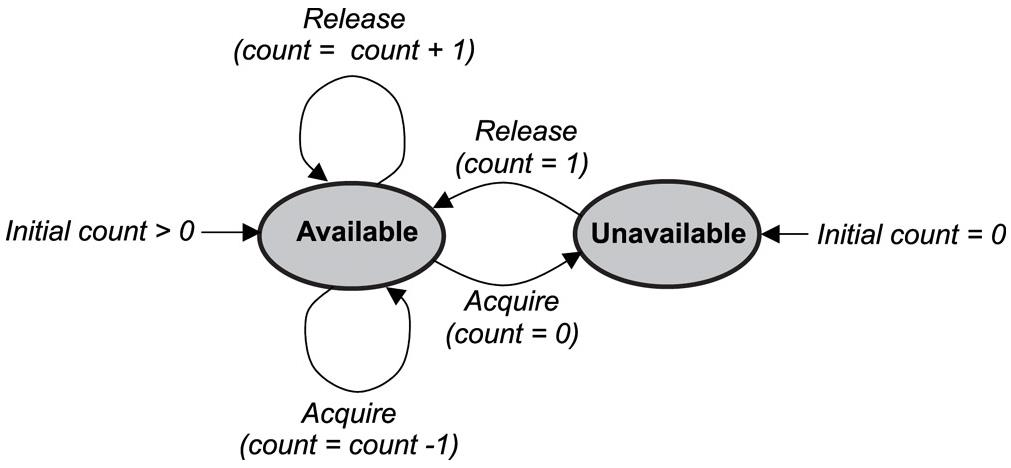
\includegraphics[width=\linewidth]{Counting_Semaphore.png}

\subsection{Mutual Exclusion (Mutex) Semaphore}

Die Mutex ist ein Sperrmechanismus (locking mechanism), welcher den Wert 0 und 1 annehmen kann.
Key words: Ownership, Recursive Locking, Task Deletion Safety, Priority Inversion Avoidance.
Recursive mutexes can be locked and unlocked multiple times by the task that owns them.

\subsection{Synchronisation}

\begin{center}
    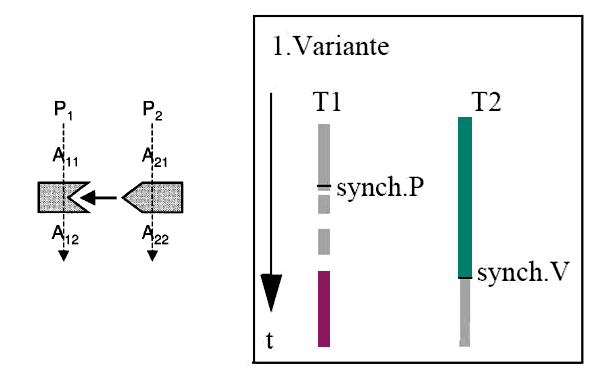
\includegraphics[width=.8\linewidth]{semaphore_sync1.png}

    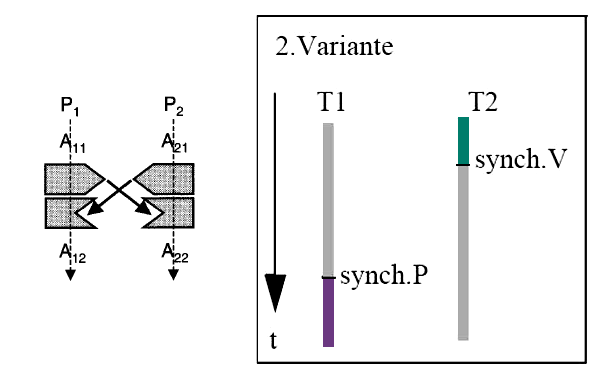
\includegraphics[width=.8\linewidth]{semaphore_sync2.png}
\end{center}


\subsection{Message Queues}

Eine Message Queue ist ein Buffer mit dem Tasks und ISR's Nachrichten austauschen und mit einander Kommuniziern können.

\subsubsection{Queue Control Block (QCB)}

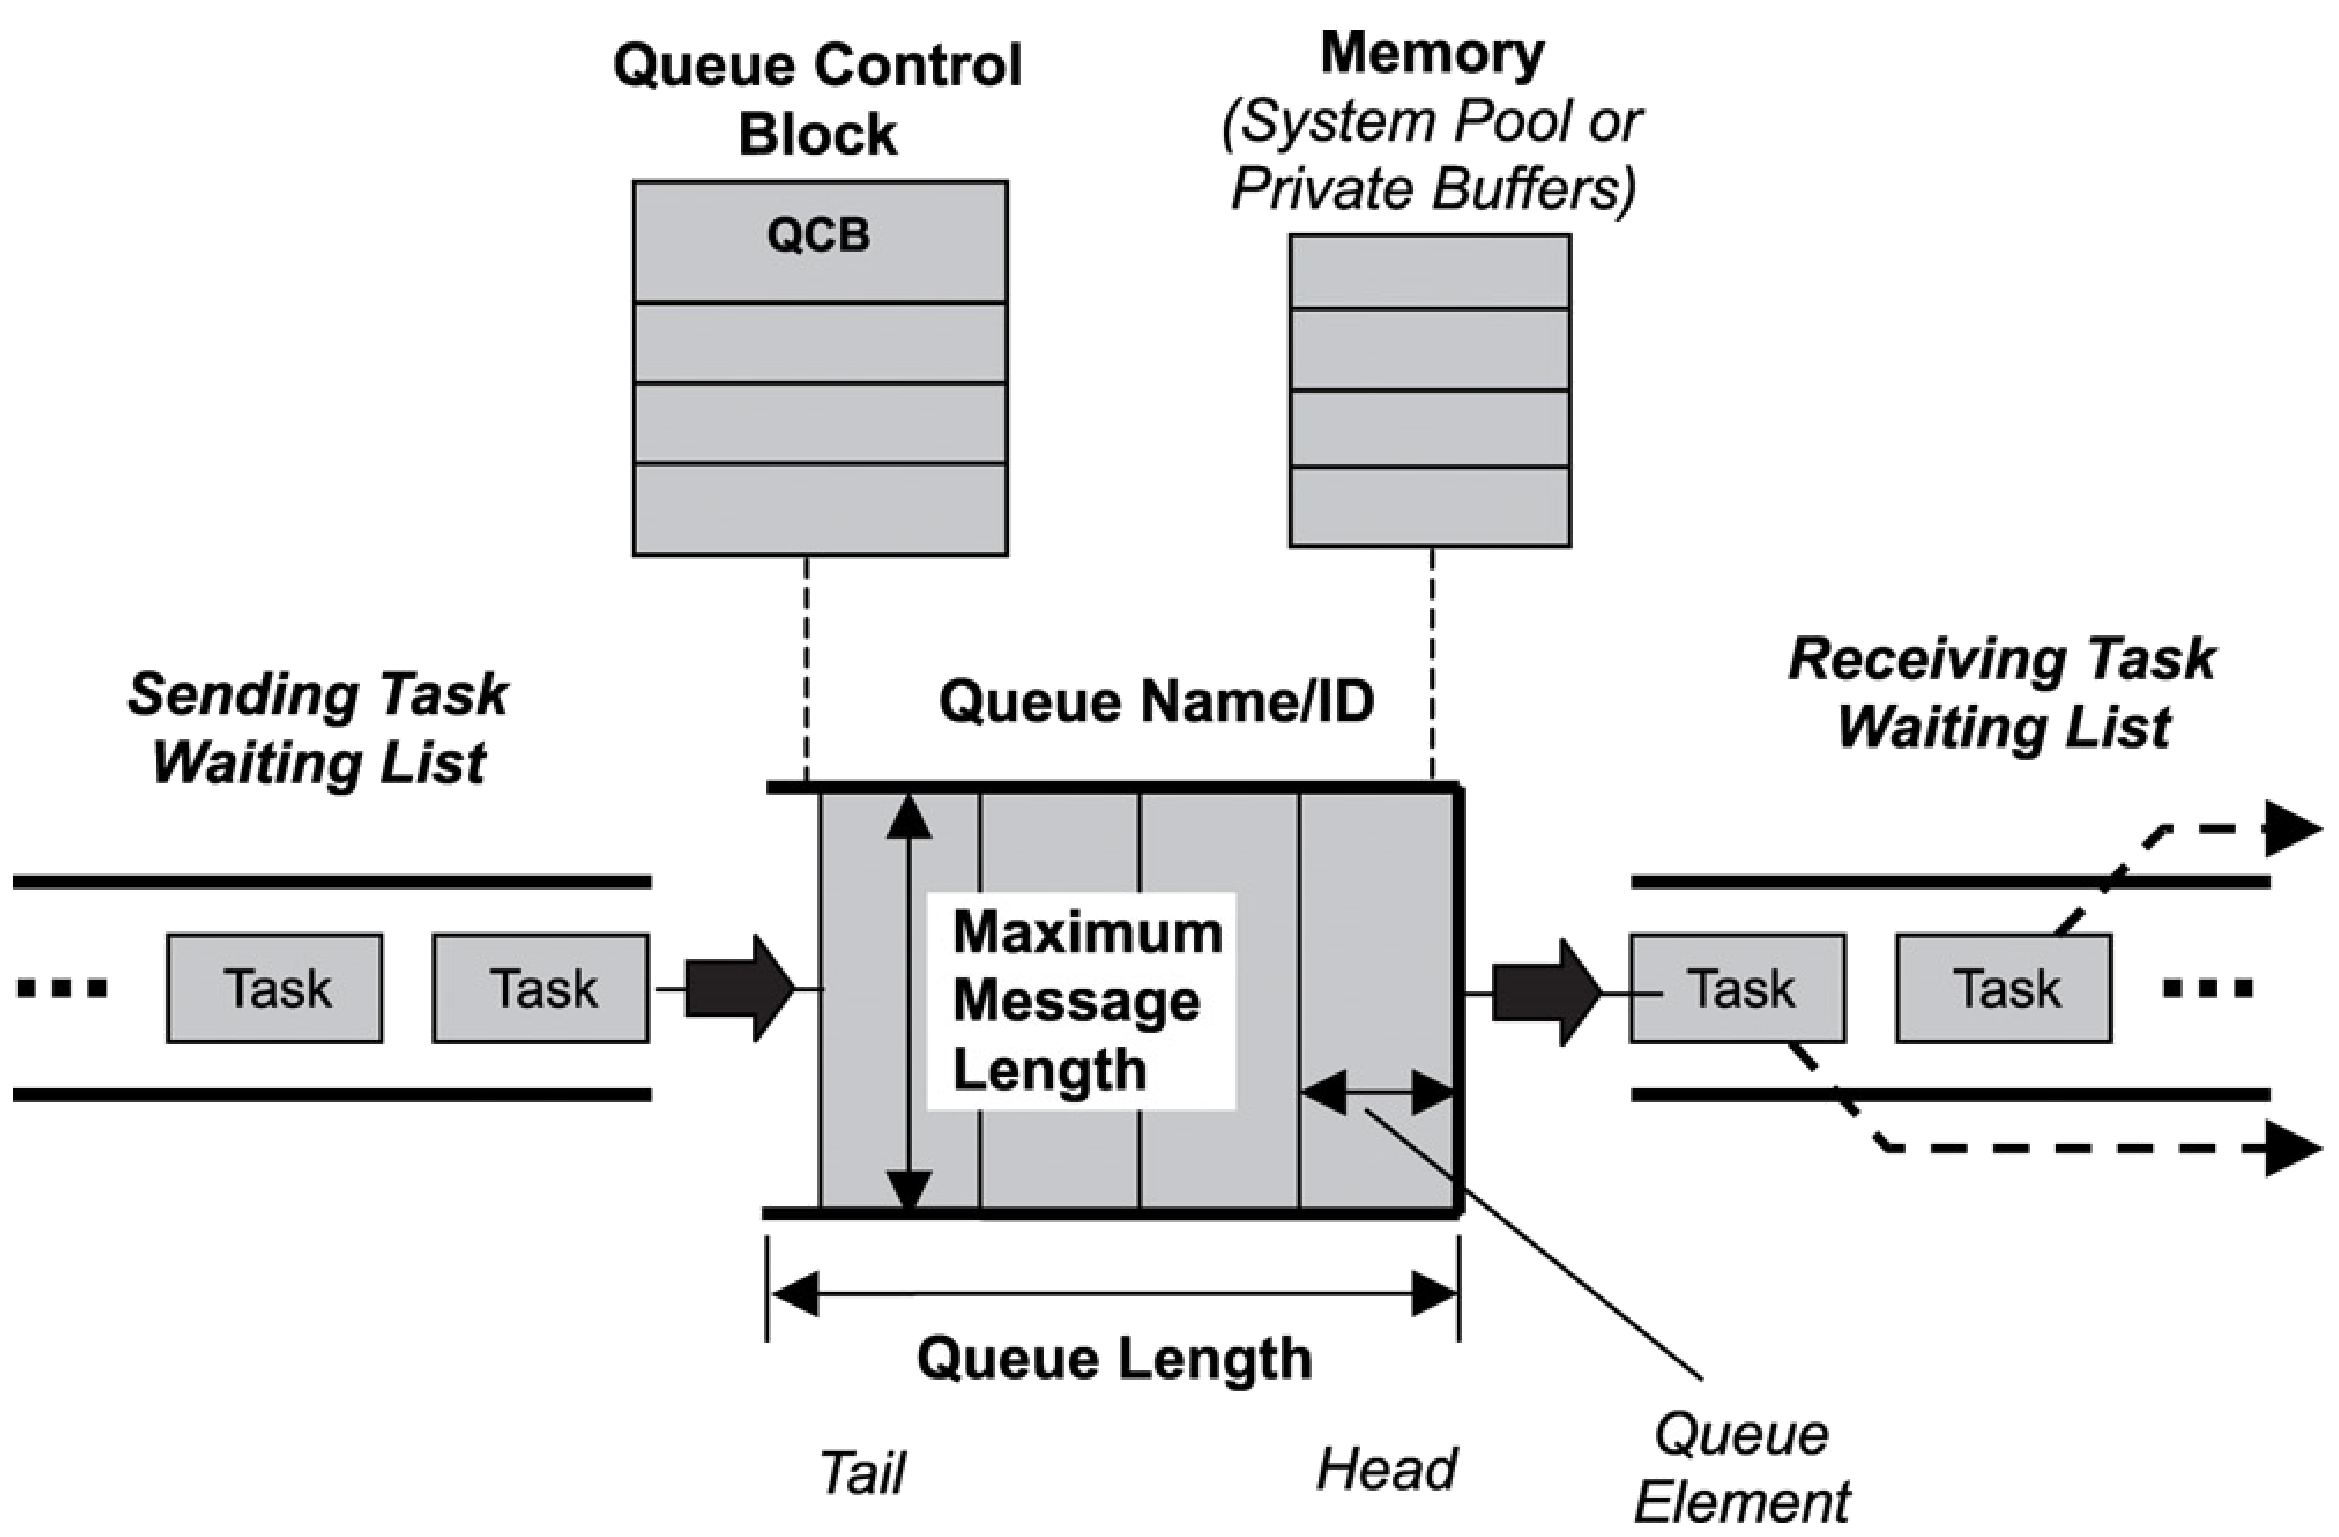
\includegraphics[width=\linewidth]{queue_control_block.png}

Zustandsdiagramm:

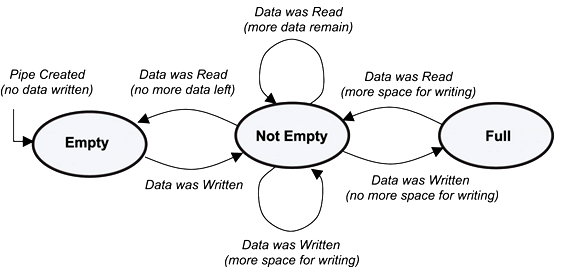
\includegraphics[width=\linewidth]{message_queue_zustandsdiagramm.png}

Unterschiedliche Kommunikationsmodelle möglich, wie One-Way Non-Interlocking und Interlocked, Two-Way Interlocked, Client-Server und Broadcast / Publish-Subscribe.


\subsubsection{Queue Set}

Queue Set ermöglicht einem RTOS Task simultan zu blockieren (pend) beim Lesezugriff auf
mehrere RTOS Queues und/oder Semaphore (block on set, not on individual object).


\subsubsection{Signals}

Ein Signal is ein Software-Interrupt welcher beim Signal-empfangenden Task einen asynchronen ablauf triggert / auslöst.
Signals can be ignored, made pending, processed (handled), or blocked.

Der \textbf{Singla Control Block} beinhaltet ein set der Signale, welche vom Task behandelt werden können.

In FreeRTOS sind Signale als \textit{Task Notifications} implementiert.


\subsubsection{Event Register, Event Groups}

Über das Event Register kann ein Task das Vorhandensein bestimmter Events prüfen,
die Einfluss auf dessen Ausführung haben können.
Eine externe Quelle, z.B. ein anderer Task oder ein ISR kann Bits im Event Register setzen,
um den Task zu informieren, dass ein bestimmter Event eingetreten ist.
Der \textbf{Event Register Control Block} ist ein Teil des \textbf{Task Control Blocks} (TCB).

In FreeRTOS is eine Event Group eine Menge von Event-Bits.
Einzelne Event-Bits innerhalb einer Event Group werden durch eine Bit-Nummer referenziert.

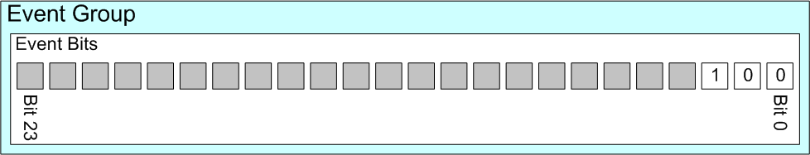
\includegraphics[width=\linewidth]{EventGroup.png}

\subsubsection{Pipes}

Pipes sind Kernel Objekte welche einen unstrukturierten Datenaustausch und Synchronisation zwischen den tasks ermöglicht.
Es können Mehrer Tasks in die pipe schreiben und auch mehrere daraus Lesen.
Pipes werden dynamisch erzeugt und gelöscht, wobei vom Kernel ein Pipe Control Block und zwei waiting lists zugewiesen werden.

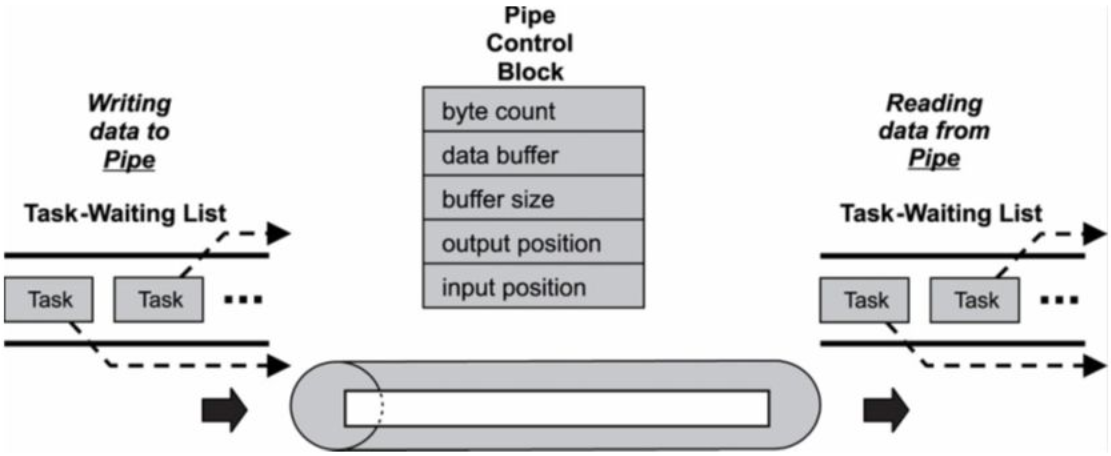
\includegraphics[width=\linewidth]{pipe_overview.png}

In FreeRTOS sind Pipes so nicht direkt vorhanden, alternativen sind Queues, Stream Buffers und Message Buffers.
	
	\newpage
\onecolumn

\section{Code Beispiele}

\subsection{Software Timer}

\underline{Software Timer API}
\lstinputlisting[firstline=0,lastline=30,style=cppstyle]{./Code/SoftwareTimer_API.c}

\underline{PWM LED}
\lstinputlisting[firstline=0,lastline=30,style=cppstyle]{./Code/SoftwareTimerPWMLED.c}


\subsection{Management von Tasks} \label{sec:task_management}

\underline{Tasks API}
\lstinputlisting[firstline=0,lastline=60,style=cppstyle]{./Code/TaskManagement_API.c}

\underline{Periodic and Aperiodic Tasks Example}
\lstinputlisting[firstline=0,lastline=60,style=cppstyle]{./Code/ManagementTasks.c}

\subsection{Semaphore} \label{sec:semaphore_api}

\underline{Semaphore API}
\lstinputlisting[firstline=0,lastline=30,style=cppstyle]{./Code/Semaphore_API.c}

\end{document}


